\documentclass[12pt]{article}
\usepackage[a4paper,width=150mm,top=25mm,bottom=25mm]{geometry}
\usepackage[spanish]{babel}
\usepackage[utf8]{inputenc}
\usepackage{csquotes}
\usepackage{amsmath}
\usepackage{graphicx}
\usepackage{caption}
\usepackage{hyperref}
\hypersetup{
    colorlinks=true,
    linkcolor=black,
    filecolor=magenta,      
    urlcolor=black,
    citecolor=black,
}
\usepackage{microtype}

\usepackage[backend=biber,style=authoryear,sorting=ynt]{biblatex}
\addbibresource{references/bibliography.bib}
\addbibresource{references/videography.bib}

\usepackage[utf8]{inputenc}

\title{La Yuxtaposición Hogar-Hospital: Transformación Espacial y Simbólica. Hospital San Juan de Dios de Bogotá}
\author{Juan Carlos Arroyo Sosa}
\date{\today}

\begin{document}

\maketitle

\begin{abstract}
Este artículo examina la yuxtaposición entre espacio doméstico e institucional en el Hospital San Juan de Dios (HSJD) de Bogotá durante su período de crisis y resistencia (2001-2017). A través del análisis de registros visuales y artísticos, se estudia cómo la apropiación de espacios hospitalarios como lugares de vida transformó la naturaleza institucional del complejo, generando una singular hibridación entre hogar y hospital. Esta investigación contribuye a la comprensión de cómo las crisis institucionales pueden catalizar transformaciones espaciales y simbólicas que desafían las categorías tradicionales de uso y significado.

\textbf{Palabras clave:} espacio hospitalario, apropiación espacial, resistencia social, memoria colectiva, transformación institucional
\end{abstract}

El Hospital San Juan de Dios de la ciudad de Bogotá fue cerrado aproximadamente en el año 1999, más de 3.600  trabajadores perdieron sus puestos fuentes de ingreso. Algunos de ellos hoy en día persisten en la resistencia al cierre y desaparición del hospital más antiguo de Sudamérica. 

La acción de diversos factores sociales, políticos, económicos y culturales llevó a este hospital a una situación recurrente de crisis y posterior cierre. Este es un caso entre muchos otros; desde la implementación de la Ley 100 de 1993 la salud pública en Colombia ha cambiado significativamente, no es la causa de todos los males, pero si resultó un detonante de síntomas a una crisis organizativa y financiera que venía de tiempo atrás.

La imagen  de un hospital que se deteriora y cierra es una imagen poderosa, es un fenómeno singular de transformación espacial donde los límites entre lo institucional y lo doméstico se desdibujan progresivamente. Los trabajadores del HSJD que permanecieron en el hospital después de su cierre oficial desarrollaron estrategias de apropiación espacial que trascendieron la mera ocupación física, creando nuevas formas de habitar el espacio hospitalario. A estos se les puede denominar síntomas visuales que maniefiestan culturales, sociales e históricas que trascienden su apariencia inmediata. El análisis revisa y categoriza en ciertos objetos y escenas dinámicas profundas esenciales para una crítica reflexiva en torno a la creación deimagen y los fenómenos sociales complejos.

Siguiendo a \cite{DidiHuberman2011}, se analiza cómo los espacios institucionales pueden transformarse en lugares de memoria y resistencia a través de la apropiación cotidiana. Así mmismo se examina cómo la yuxtaposición de usos genera nuevas capas de significado en los espacios institucionales. 

Los registros visuales analizados evidencian una progresiva domesticación de espacios originalmente clínicos. Las salas de espera se convirtieron en salas de estar, los consultorios en dormitorios, y los pasillos en espacios de socialización. Un aspecto recurrente es el encuadre de lugares y objetos deteriorados por el tiempo: las imágenes evidencian el triunfo del agua, el musgo y la hierba sobre las superficies. Esta característica visible contrasta con el impulso de quienes han resistido y cuidado el San Juan, personas que han luchado a contracorriente mediante actos de expresión visualmente documentados, generando impulsos de resistencia ante la hostilidad del contexto y las circunstancias.

\begin{figure}[h]
    \centering
    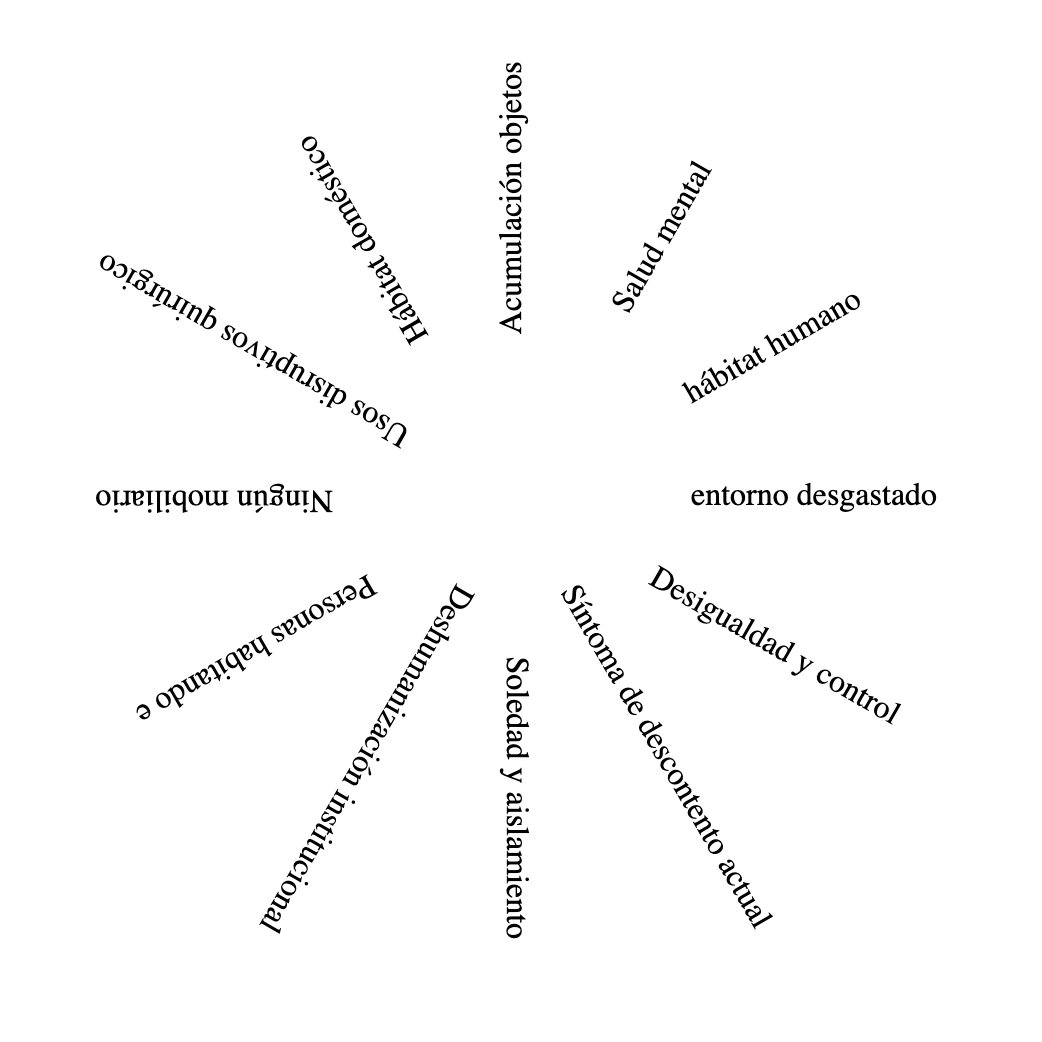
\includegraphics[width=\textwidth]{images/category1.png}
    \caption{visualización radial 1}
    \label{fig:category1}
\end{figure}

La yuxtaposición hogar-hospital generó nuevas categorías espaciales donde los objetos médicos coexisten con elementos domésticos, creando un paisaje visual único que refleja la resistencia social. La transformación espacial actuó como estrategia de resistencia, permitiendo a los trabajadores mantener su vínculo con la institución mientras adaptaban los espacios a sus necesidades cotidianas.

La yuxtaposición hogar-hospital en el HSJD representa un caso paradigmático de cómo las crisis institucionales pueden generar nuevas formas de habitar y significar los espacios. Como señala \cite{Castiblanco2017}, estas transformaciones espaciales no son meras adaptaciones funcionales, sino manifestaciones de resistencia que cuestionan las categorías tradicionales de uso institucional catalizando una transformación espacial que desafió los límites tradicionales entre lo público y lo privado. Las apropiaciones domésticas de espacios hospitalarios a largo plazo a través de los registros testimoniales, argumetales, documentales y performativos derivaron en resonancias o ecos de refleción y preservación de la memoria en obras de creación derivadas o conexas a dicha experiencia vital.

\begin{figure}[h]
    \centering
    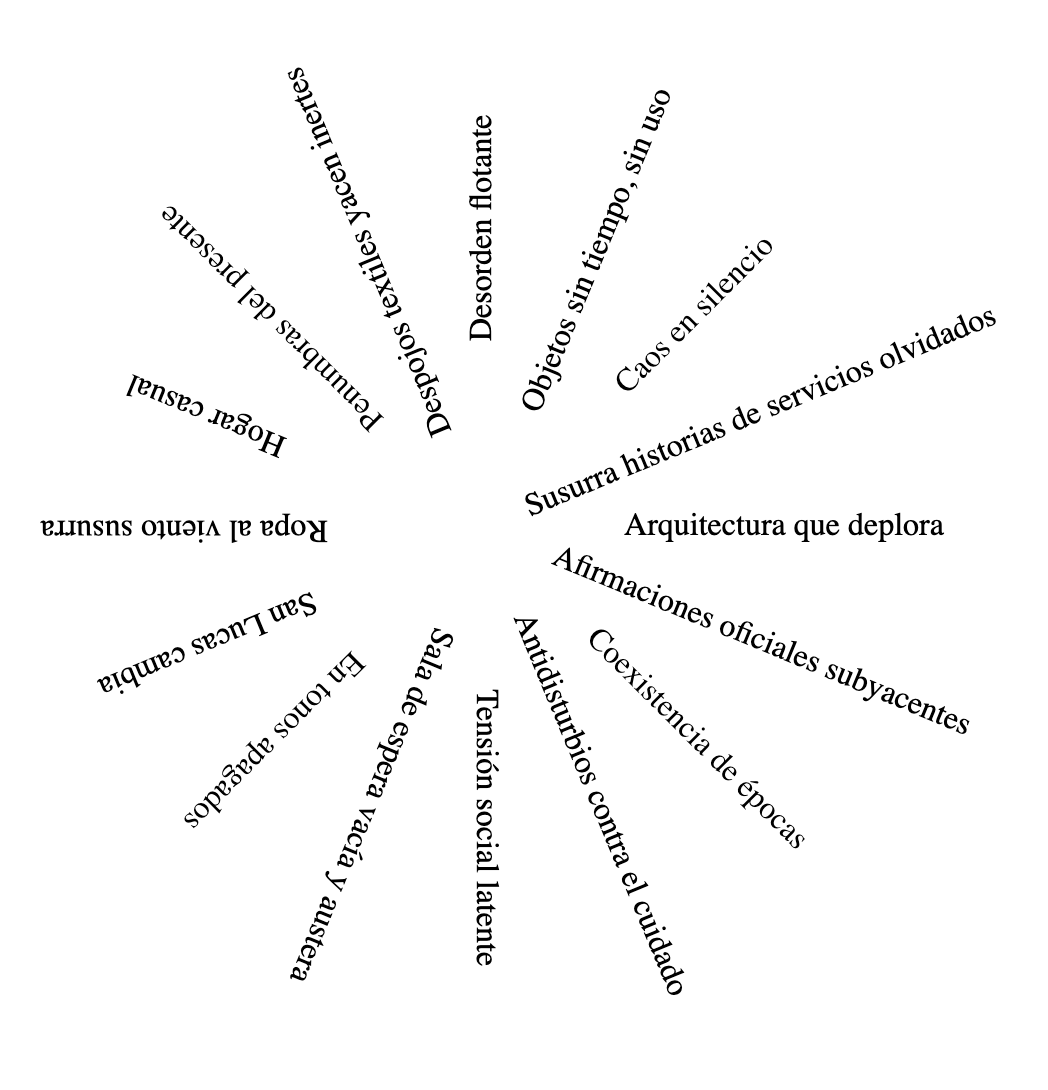
\includegraphics[width=\textwidth]{images/category2.png}
    \caption{visualización radial 2}
    \label{fig:category2}
\end{figure}


El fenómeno sociocomunicativo del caso de estudio se manifiesta a través de elementos anacrónicos que atraviesan la imagen no-domesticada - aquella que se desprende de propósitos publicitarios o periodísticos - y se integra en redes dialógicas no-textuales mediante el montaje con otros discursos visuales. Esta interacción facilita la emergencia de la imagen-síntoma y los indicios de anacronismos.

\bibliographystyle{plain}
\bibliography{references}

\printbibliography

\end{document}
